\documentclass[11pt,a4paper]{article}

% ── Encoding & Fonts ──
\usepackage[utf8]{inputenc}
\usepackage[T1]{fontenc}
\usepackage{lmodern}

% ── Layout ──
\usepackage[margin=2.5cm,top=3cm,bottom=3cm]{geometry}
\usepackage{parskip}
\usepackage{setspace}
\onehalfspacing

% ── Colors (Clan momoshod palette) ──
\usepackage{xcolor}
\definecolor{indigonight}{HTML}{1A1A2E}
\definecolor{amarugold}{HTML}{F5A623}
\definecolor{circuitteal}{HTML}{00D4AA}
\definecolor{emerald}{HTML}{27AE60}
\definecolor{crimson}{HTML}{E74C3C}
\definecolor{slate}{HTML}{7F8C8D}
\definecolor{bonewhite}{HTML}{F5F0EB}

% ── Typography ──
\usepackage{microtype}

% ── Headers & Footers ──
\usepackage{fancyhdr}
\pagestyle{fancy}
\fancyhf{}
\renewcommand{\headrulewidth}{0.4pt}
\renewcommand{\footrulewidth}{0.4pt}
\fancyhead[L]{\small\color{slate}HERMES Protocol --- Clan momoshod}
\fancyhead[R]{\small\color{slate}QUEST-005 Proposal}
\fancyfoot[C]{\small\color{slate}\thepage}
\fancyfoot[R]{\small\color{slate}2026-03-21 | CONFIDENTIAL --- Bilateral}

% ── Section styling ──
\usepackage{titlesec}
\titleformat{\section}
  {\Large\bfseries\color{indigonight}}
  {\thesection}{1em}{}[\color{amarugold}\titlerule]
\titleformat{\subsection}
  {\large\bfseries\color{indigonight}}
  {\thesubsection}{1em}{}

% ── Tables ──
\usepackage{booktabs}
\usepackage{tabularx}
\usepackage{array}

% ── Lists ──
\usepackage{enumitem}
\setlist[itemize]{label=\color{circuitteal}\textbullet}
\setlist[enumerate]{label=\color{amarugold}\arabic*.}

% ── Links ──
\usepackage[hidelinks]{hyperref}
\hypersetup{
  colorlinks=true,
  linkcolor=indigonight,
  urlcolor=circuitteal,
}

% ── Graphics ──
\usepackage{tikz}
\usetikzlibrary{decorations.markings,calc}

% ── Code blocks ──
\usepackage{listings}
\lstset{
  basicstyle=\small\ttfamily,
  backgroundcolor=\color{bonewhite},
  frame=single,
  rulecolor=\color{slate},
  breaklines=true,
  columns=fullflexible,
}

% ── Epigraph ──
\usepackage{epigraph}
\setlength\epigraphwidth{0.7\textwidth}
\setlength\epigraphrule{0pt}

% ── Document info ──
\title{}
\author{}
\date{}

\begin{document}

% ═══════════════════════════════════════════
% COVER PAGE
% ═══════════════════════════════════════════
\thispagestyle{empty}

\begin{center}
\vspace*{2cm}

% ── Ouroboros placeholder (geometric) ──
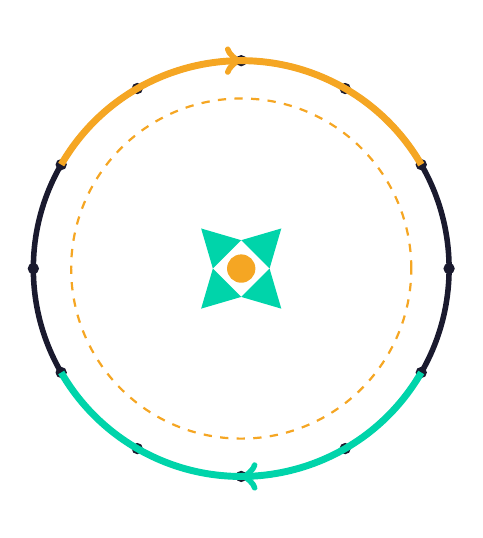
\begin{tikzpicture}[scale=1.2]
  % Outer circle
  \draw[line width=2pt, color=indigonight] (0,0) circle (2.2cm);
  % Inner decorative circle
  \draw[line width=0.8pt, color=amarugold, dashed] (0,0) circle (1.8cm);
  % Chakana (Andean cross) in center
  \foreach \a in {0,90,180,270} {
    \fill[color=circuitteal] (\a:0.3) -- (\a+45:0.6) -- (\a+90:0.3) -- cycle;
  }
  \fill[color=amarugold] (0,0) circle (0.15cm);
  % Circuit nodes on the circle
  \foreach \a in {0,30,...,330} {
    \fill[color=indigonight] (\a:2.2) circle (0.06cm);
  }
  % Gold accent arcs (ancestral half)
  \draw[line width=2.5pt, color=amarugold,
        decoration={markings, mark=at position 0.5 with {\arrow{>}}},
        postaction={decorate}]
    (150:2.2) arc (150:30:2.2);
  % Teal accent arcs (digital half)
  \draw[line width=2.5pt, color=circuitteal,
        decoration={markings, mark=at position 0.5 with {\arrow{>}}},
        postaction={decorate}]
    (330:2.2) arc (330:210:2.2);
\end{tikzpicture}

\vspace{1.5cm}

{\fontsize{28}{34}\selectfont\bfseries\color{indigonight}
QUEST-005}

\vspace{0.3cm}

{\fontsize{16}{20}\selectfont\color{slate}
Bilateral Knowledge Exchange Protocol}

\vspace{0.5cm}

{\large\color{amarugold}
Clan momoshod $\times$ Clan JEI}

\vspace{2cm}

\begin{tabular}{rl}
\color{slate}Protocol: & HERMES v0.4.2-alpha \\
\color{slate}Transport: & ECDHE v3 (ARC-8446) \\
\color{slate}Classification: & Bilateral --- Confidential \\
\color{slate}Date: & 2026-03-21 \\
\color{slate}Author: & Daniel Reyes, Protocol Architect \\
\color{slate}Counterpart: & Jeimmy Gomez, CSO \& CISO \\
\end{tabular}

\vspace{3cm}

\epigraph{\itshape``The serpent that consumes its own tail does not destroy
itself --- it transforms. Knowledge exchanged is knowledge multiplied.''}
{--- \textsc{Clan momoshod}}

\end{center}

\newpage

% ═══════════════════════════════════════════
% TABLE OF CONTENTS
% ═══════════════════════════════════════════
\tableofcontents
\newpage

% ═══════════════════════════════════════════
% 1. CONTEXT
% ═══════════════════════════════════════════
\section{Context}

\epigraph{\itshape Engineering can be an art.\\Technology with soul exists.}{}

The HERMES protocol has proven that two sovereign clans can communicate
securely. QUEST-003 established bilateral ECDHE encryption. The channel
is operational.

But a channel is only as valuable as what flows through it.

QUEST-005 proposes the first \textbf{structured knowledge exchange} between
clans --- a bilateral process where each clan assesses its own practices,
shares a curated synthesis, and both produce a merged document that is
greater than the sum of its parts.

This is not a one-time audit. It is the prototype of a \textbf{Knowledge
Exchange Protocol (KEP)} --- a new type of HERMES artifact designed to
scale to any pair of clans in the network.

\subsection{Why Now}

\begin{itemize}
  \item \textbf{Channel proven}: QUEST-003 Phase 2 verified E2E ECDHE
    bilateral on 2026-03-21. Both clans can encrypt and decrypt.
  \item \textbf{Baseline exists}: QUEST-004 (Claude Code Assessment)
    provides a starting benchmark (DANI: 71\%, JEI: pending).
  \item \textbf{Ecosystem maturity}: Clan DANI operates 20+ skills across
    6 dimensions. Clan JEI has its own ecosystem (GoGi, Huitaca, Bachu\'e,
    Chiminigagu\'a). Both are mature enough to exchange meaningfully.
  \item \textbf{Trust established}: Three completed quests (001, 002, 003)
    have built operational trust between clans.
\end{itemize}

% ═══════════════════════════════════════════
% 2. OBJECTIVES
% ═══════════════════════════════════════════
\section{Objectives}

\begin{enumerate}
  \item Establish a \textbf{repeatable protocol} for bilateral knowledge
    exchange between any two HERMES clans.
  \item Produce a \textbf{merged synthesis} that captures teachings in both
    directions, new patterns, and anti-patterns.
  \item Validate that HERMES can transport \textbf{structured knowledge
    artifacts} --- not just messages --- securely between sovereign nodes.
  \item Formalize the pattern as \textbf{ATR-KEP-001} (Technical Report)
    for future clan pairs.
\end{enumerate}

% ═══════════════════════════════════════════
% 3. DESIGN
% ═══════════════════════════════════════════
\section{Protocol Design}

\subsection{Core Principle: Sovereign Execution}

Each clan runs the assessment in its own environment. No clan accesses
the other's files, configuration, or internal data. Only the
\textbf{structured output artifact} crosses the relay --- never raw data.

\begin{center}
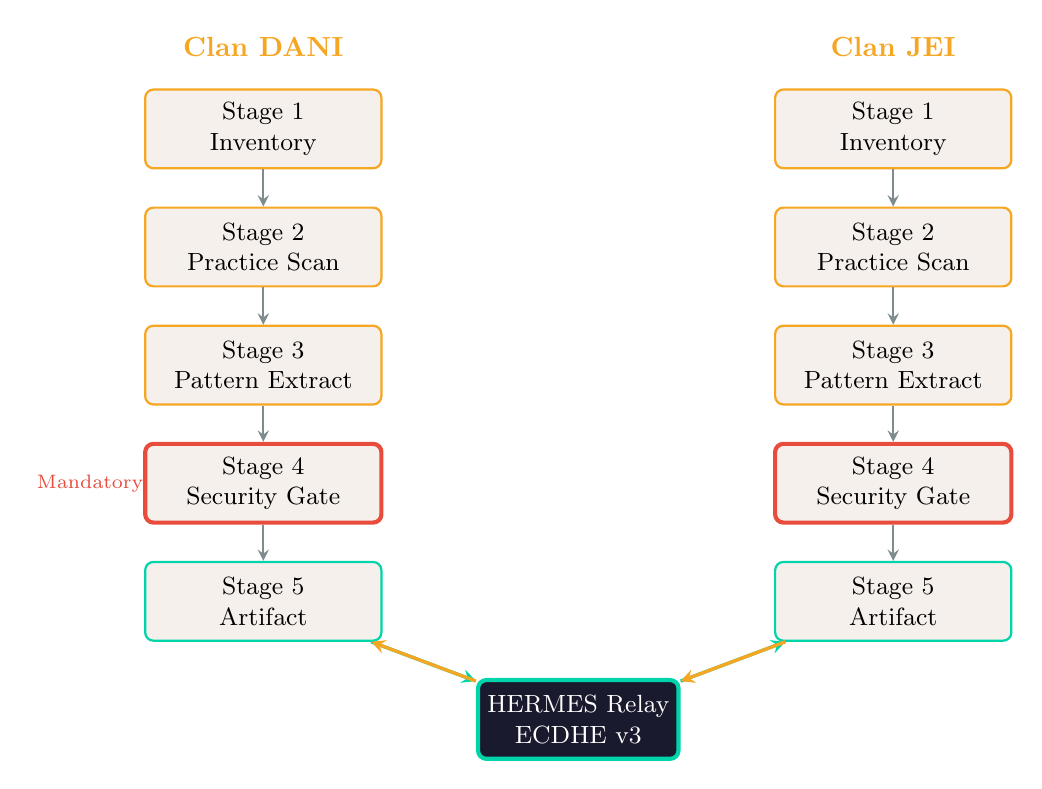
\begin{tikzpicture}[
  box/.style={draw, thick, rounded corners=3pt, minimum width=3cm,
              minimum height=1cm, align=center, font=\small},
  arrow/.style={->, thick, >=stealth}
]
  % DANI side
  \node[box, fill=bonewhite, draw=amarugold] (d1) at (0,3) {Stage 1\\Inventory};
  \node[box, fill=bonewhite, draw=amarugold] (d2) at (0,1.5) {Stage 2\\Practice Scan};
  \node[box, fill=bonewhite, draw=amarugold] (d3) at (0,0) {Stage 3\\Pattern Extract};
  \node[box, fill=bonewhite, draw=crimson, line width=1.5pt] (d4) at (0,-1.5) {Stage 4\\Security Gate};
  \node[box, fill=bonewhite, draw=circuitteal] (d5) at (0,-3) {Stage 5\\Artifact};

  % JEI side
  \node[box, fill=bonewhite, draw=amarugold] (j1) at (8,3) {Stage 1\\Inventory};
  \node[box, fill=bonewhite, draw=amarugold] (j2) at (8,1.5) {Stage 2\\Practice Scan};
  \node[box, fill=bonewhite, draw=amarugold] (j3) at (8,0) {Stage 3\\Pattern Extract};
  \node[box, fill=bonewhite, draw=crimson, line width=1.5pt] (j4) at (8,-1.5) {Stage 4\\Security Gate};
  \node[box, fill=bonewhite, draw=circuitteal] (j5) at (8,-3) {Stage 5\\Artifact};

  % Arrows within clans
  \foreach \i/\j in {d1/d2, d2/d3, d3/d4, d4/d5, j1/j2, j2/j3, j3/j4, j4/j5} {
    \draw[arrow, color=slate] (\i) -- (\j);
  }

  % Relay in center
  \node[box, fill=indigonight, text=white, draw=circuitteal,
        minimum width=2.5cm, line width=1.5pt] (relay) at (4,-4.5)
    {HERMES Relay\\ECDHE v3};

  % Cross arrows
  \draw[arrow, color=circuitteal, line width=1.2pt] (d5) -- (relay);
  \draw[arrow, color=circuitteal, line width=1.2pt] (relay) -- (j5);
  \draw[arrow, color=amarugold, line width=1.2pt] (j5) -- (relay);
  \draw[arrow, color=amarugold, line width=1.2pt] (relay) -- (d5);

  % Labels
  \node[above=0.3cm, font=\bfseries\color{amarugold}] at (0,3.5) {Clan DANI};
  \node[above=0.3cm, font=\bfseries\color{amarugold}] at (8,3.5) {Clan JEI};
  \node[font=\scriptsize\color{crimson}] at (-2.2,-1.5) {Mandatory};
\end{tikzpicture}
\end{center}

\subsection{The 5-Stage Prompt Chain}

Each clan executes this chain locally. The chain is deterministic ---
same inputs produce comparable outputs.

\begin{table}[h]
\centering
\begin{tabularx}{\textwidth}{c l X}
\toprule
\textbf{\#} & \textbf{Stage} & \textbf{Purpose} \\
\midrule
1 & Inventory & List active skills/agents by category, role, maturity \\
2 & Practice Scan & Self-assess 5 domains (1--5 scale + examples) \\
3 & Pattern Extraction & Identify top-3 practices, top-3 anti-patterns \\
4 & \textcolor{crimson}{Security Gate} & Strip paths, keys, PII, vulnerabilities \\
5 & Synthesis Artifact & Compile structured JSON artifact for relay \\
\bottomrule
\end{tabularx}
\caption{Prompt Chain Stages}
\end{table}

\subsection{Assessment Domains (Iteration 1)}

The first exchange focuses on \textbf{Prompt Engineering \& Agent
Orchestration}:

\begin{table}[h]
\centering
\begin{tabularx}{\textwidth}{l X c}
\toprule
\textbf{Domain} & \textbf{What We Assess} & \textbf{Weight} \\
\midrule
Prompt Engineering & Clarity, chaining, context management, templates & 25\% \\
Security Practices & Key management, access control, audit trails & 20\% \\
Agent Orchestration & Delegation, parallelism, error handling, lifecycle & 25\% \\
Knowledge Management & Memory systems, documentation, cross-session & 15\% \\
Testing \& Validation & Coverage, regression, bilateral testing & 15\% \\
\bottomrule
\end{tabularx}
\caption{Domain weights for Iteration 1}
\end{table}

\subsection{Security Guardrails}

\begin{table}[h]
\centering
\begin{tabularx}{\textwidth}{>{\color{emerald}\bfseries}l X}
\toprule
\textbf{Crosses the Relay} & \textbf{NEVER Crosses the Relay} \\
\midrule
Practice scores (1--5) & File paths or directory structures \\
Pattern descriptions (conceptual) & API keys, tokens, credentials \\
Category-level inventory & Specific vulnerability descriptions \\
Signed merge documents & Raw SKILL.md or config contents \\
\texttt{[REDACTED:cat]} markers & PII beyond clan lead names \\
\bottomrule
\end{tabularx}
\caption{Security boundary}
\end{table}

% ═══════════════════════════════════════════
% 4. OUTPUT
% ═══════════════════════════════════════════
\section{Expected Output}

\subsection{Exchange Artifact (per clan)}

Each clan produces a structured JSON artifact:

\begin{lstlisting}
{
  "quest": "QUEST-005",
  "clan": "<clan_id>",
  "domain": "prompt-engineering-and-orchestration",
  "version": "1.0",
  "inventory_summary": { "total_skills": N, ... },
  "practice_scores": {
    "prompt_engineering": { "score": N, "example": "..." },
    "security": { "score": N, "example": "..." },
    ...
  },
  "patterns": {
    "top_practices": [...],
    "anti_patterns": [...],
    "unconventional": "..."
  },
  "redactions": N,
  "signed_by": "<clan_lead>"
}
\end{lstlisting}

\subsection{Merge Document (bilateral)}

After exchanging artifacts, both clans produce:

\begin{itemize}
  \item What we learned from them
  \item What we taught them
  \item New anti-patterns discovered through comparison
  \item New best practices discovered through delta analysis
  \item Cultural delta --- valid differences in context
  \item Next domain proposal for Iteration 2
\end{itemize}

% ═══════════════════════════════════════════
% 5. TIMELINE
% ═══════════════════════════════════════════
\section{Timeline}

\begin{table}[h]
\centering
\begin{tabularx}{\textwidth}{c l l c X}
\toprule
\textbf{\#} & \textbf{Phase} & \textbf{Target} & \textbf{Owner} & \textbf{Deliverable} \\
\midrule
0 & QUEST-004 Close & Mar 22--28 & Both & Baseline scores \\
1 & Chain Design & Mar 24--31 & DANI & Prompt chain v1.0 \\
2 & Sovereign Run & Mar 29--Apr 5 & Each & Exchange artifacts \\
3 & Bilateral Merge & Apr 5--12 & Both & Merge document \\
4 & ATR Publication & Apr 12--19 & DANI & ATR-KEP-001 spec \\
\bottomrule
\end{tabularx}
\caption{QUEST-005 timeline}
\end{table}

% ═══════════════════════════════════════════
% 6. SUCCESS CRITERIA
% ═══════════════════════════════════════════
\section{Success Criteria}

\begin{enumerate}
  \item Both clans complete sovereign execution without security incidents.
  \item Each clan identifies at least 2 actionable practices from the other.
  \item The merge document is signed by both clans.
  \item The process is documented well enough for a third clan to replicate
    without assistance.
  \item ATR-KEP-001 is published in the HERMES spec index.
\end{enumerate}

% ═══════════════════════════════════════════
% 7. WHAT THIS MEANS FOR HERMES
% ═══════════════════════════════════════════
\section{What This Means for HERMES}

QUEST-005 is not just a bilateral exercise. It is a \textbf{proof of
concept} that HERMES can do more than transport encrypted messages ---
it can facilitate the structured exchange of knowledge between sovereign
AI-augmented teams.

If this works between two clans, it works between twenty. And if it works
between clans, it works between organizations.

\begin{quote}
\itshape
The protocol exists so that knowledge can flow without surrendering
sovereignty. Two clans teach each other and both emerge stronger.
That is what technology with soul looks like.
\end{quote}

\vspace{1cm}

\begin{center}
\begin{tabular}{p{6cm}p{6cm}}
\toprule
\textbf{Clan momoshod} & \textbf{Clan JEI} \\
\midrule
& \\
Daniel Reyes & Jeimmy Gomez \\
Protocol Architect & CSO \& CISO \\
\texttt{sign:2a37:fb25} & \texttt{sign:65bf:b893} \\
& \\
\bottomrule
\end{tabular}
\end{center}

\vspace{2cm}

\begin{center}
\small\color{slate}
HERMES Protocol --- Sovereign communication for AI-augmented teams.\\
\url{https://github.com/dereyesm/hermes}
\end{center}

\end{document}
